\chapter{Anormale Diffusion - Lorentz-Modell}

Zum Abschluss soll das Diffusionsverhalten von Teilchen untersucht werden, die auf den Porenraum des Boolschen Modells beschr�nkt sind. Die Visualisierung der Teilchentrajektorie eines Testteilchens mit Radius $\sigma = 0.1$ ist in \fref{fig:big} zu sehen.

\begin{figure}[htbp]
	\centering
		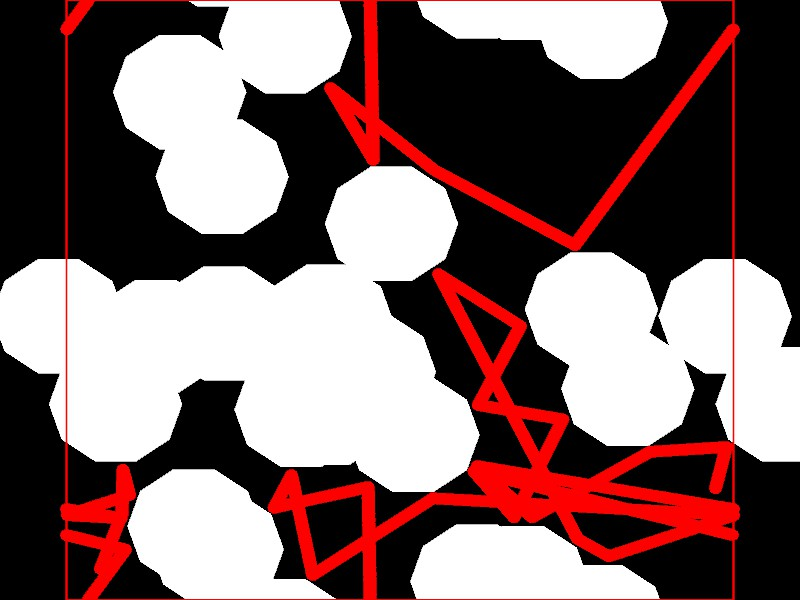
\includegraphics[width=0.70\textwidth]{img/big.jpg}
	\caption{Teilchentrajektorie im Porenraum des Boolschen Modells f�r ein Teilchen mit Radius $\sigma = 0.1$}
	\label{fig:big}
\end{figure}

Die erste Frage, die sich stellt, ist, ob sich die Trajektorie �ndert, wenn man Punktteilchen betrachtet und daf�r den Radius der Scheiben, die die Hindernisse darstellen, auf $R=R+\sigma$ vergr��ert. Da f�r die St��e mit den Hindernisteilchen vollkommen elastische St��e angenommen werden, f�hrt diese �nderung zu den gleichen Trajektorien (siehe \fref{fig:small}). Durch das gleiche Argument spielt auch der Betrag der Anfangsgeschwindigkeit der Teilchen keine Rolle. Die Teilchen legen zwar insgesamt f�r h�here Anfangsgeschwindigkeiten weitere Wege zur�ck, aber das Abprallverhalten an den Hindernisse bleibt das gleiche.

\begin{figure}[htbp]
	\centering
		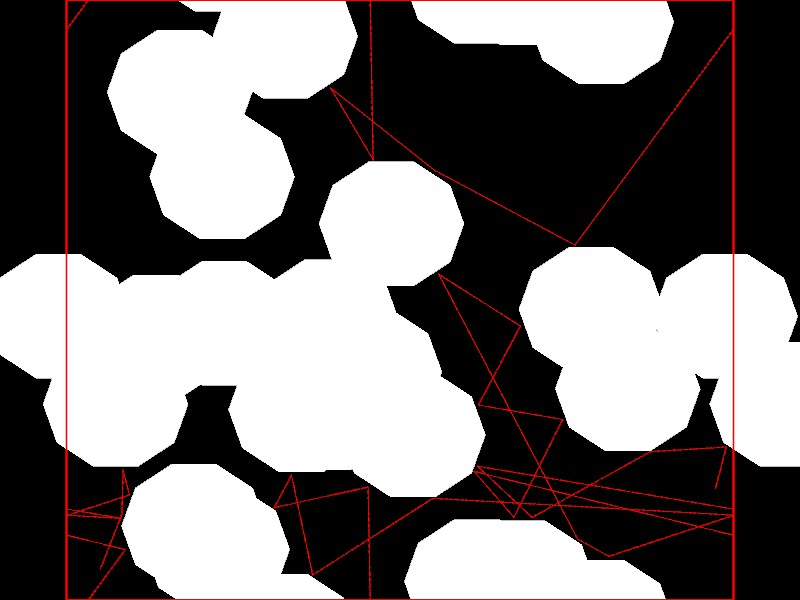
\includegraphics[width=0.70\textwidth]{img/small.jpg}
	\caption{Die Gr��e der Testteilchen spielt keine Rolle, wenn die Gr��e der Hindernisse angepasst wird (vgl \fref{fig:big}).}
	\label{fig:small}
\end{figure}